\section{Descriptive Data Analysis}

\subsection{Dataset Overview}

A dataset, comprising a combination of historical sales data of Wolt and Foodora, is used in this study. The sample size was mostly restricted to one vendor because it was not possible to reach various branches. The study can be further extended with more data. Foodora, on the other hand, is any other competitive party of the existing delivery services.

The final dataset, having been cleaned and integrated, is a structured, transaction record, which is analyzed and developed into a model. The database comprises of a total number of records of individual orders during the period of time chosen. A record is associated with every transaction and it contains details regarding sales and time.

The dataset contains several key variables. They usually include order date and time, sales value, platform identifier (Wolt or Foodora), and other features that are developed in the course of preprocessing, including day of the week or month. Patterns are analyzed with these variables and help to predict models.

The data includes a certain period of time, and the study enables the researcher to record the trends and seasonal changes in the demand. This window is critical in determining the customer behavior changes and making sure that the forecasting models are trained of adequate historical information. 

All in all, the data set gives a full picture of the platform-level sales activity and is the foundation of descriptive analysis, forecasting and optimization in this research.


\subsection{Sales Patterns}

This section analyzes the historical sales data to identify important patterns in customer demand. Understanding these patterns helps in building accurate forecasting models and supports better decision-making.

\begin{table}[h]
\centering
\begin{tabular}{|p{4cm}|p{10cm}|}
\hline
\textbf{Category} & \textbf{Description} \\
\hline
Daily Order Trends & Shows how the number of orders changes day by day. It helps identify fluctuations in demand, including peaks and low periods influenced by factors such as promotions, holidays, or external events. \\
\hline
Weekly Patterns & Examines how demand varies across different days of the week. Typically, higher demand is observed on weekends, while weekdays show more stable but lower demand. This helps capture weekly seasonality. \\
\hline
Platform Comparison & Compares sales performance between Wolt and Foodora. It highlights differences in order volume, trends, and platform-specific demand, supporting better platform-level decision-making. \\
\hline
\end{tabular}
\caption{Summary of Sales Patterns}
\end{table}


\subsection{Exploratory Data Analysis (EDA)}

Exploratory Data Analysis (EDA) is done to understand the characteristics of the dataset, and to find out the key relationship between the data. It helps to visualize behavior of orders with time and helps to choose appropriate forecasting models.


In this study, various graphical analyses are employed. First is How are Order Values Distributed over Different Transactions while Being Associated with Orders. This help in checking if the data is skewed or either outliers.


Second, the order volatility of the networks is explored to investigate to what extent demand changes with time. Very high volatility means volatile demand while low volatility means the ordering patterns are more stable. Volatility is an important concept, to measure the difficulty of predicting.


Third, trend patterns are explored using time series plots. These plots show the volume of orders as a function of time and help to identify long-term trends, seasonal effects, and sudden shifts in demand. The historical order trend from the dataset we analyzed is shown in Fig.~\ref{fig:historical_orders}. The graph displays demand over time, showing demand patterns, peaks, drops, and seasonality among others.

Overall, the EDA provides valuable insights into the structure and behavior of the data, forming the foundation for the forecasting and optimization steps in this study.


\begin{figure}[h]
\centering
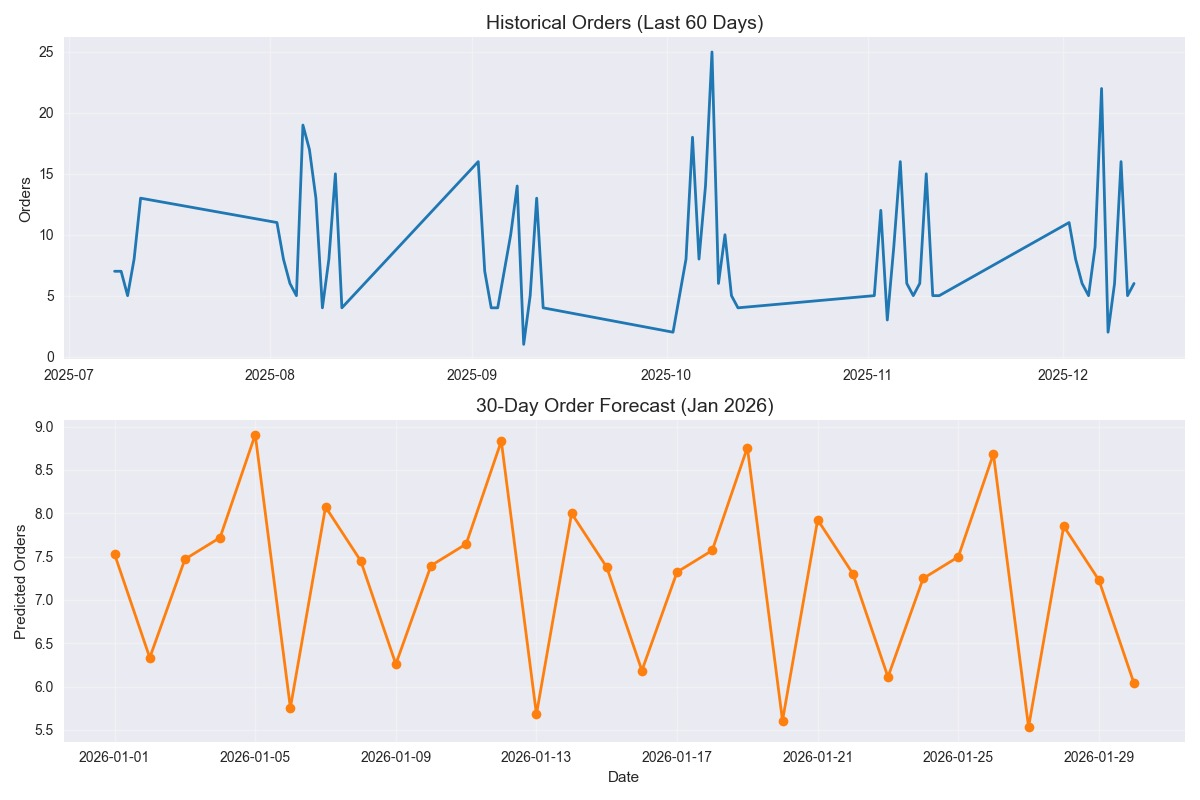
\includegraphics[width=0.9\textwidth]{figures/1.jpeg}
\caption{Historical Order Trends}
\label{fig:historical_orders}
\end{figure}